%%%%%%%%%%%%%%%%%%%%%%%%%%%%%%%%%%%%%%%
% Wenneker Resume/CV
% LaTeX Template
% Version 1.1 (19/6/2016)
%
% This template has been downloaded from:
% http://www.LaTeXTemplates.com
%
% Original author:
% Frits Wenneker (http://www.howtotex.com) with extensive modifications by 
% Vel (vel@LaTeXTemplates.com)
%
% License:
% CC BY-NC-SA 3.0 (http://creativecommons.org/licenses/by-nc-sa/3.0/
%
%%%%%%%%%%%%%%%%%%%%%%%%%%%%%%%%%%%%%%

%----------------------------------------------------------------------------------------
%	PACKAGES AND OTHER DOCUMENT CONFIGURATIONS
%----------------------------------------------------------------------------------------

\documentclass[a4paper,12pt]{article} % Font and paper size, changed from memoir to article

%%%%%%%%%%%%%%%%%%%%%%%%%%%%%%%%%%%%%%%%%
% Wenneker Resume/CV
% Structure Specification File
% Version 1.1 (19/6/2016)
%
% This file has been downloaded from:
% http://www.LaTeXTemplates.com
%
% Original author:
% Frits Wenneker (http://www.howtotex.com) with extensive modifications by 
% Vel (vel@latextemplates.com)
%
% License:
% CC BY-NC-SA 3.0 (http://creativecommons.org/licenses/by-nc-sa/3.0/)
%
%%%%%%%%%%%%%%%%%%%%%%%%%%%%%%%%%%%%%%%%%

%----------------------------------------------------------------------------------------
%	PACKAGES AND OTHER DOCUMENT CONFIGURATIONS
%----------------------------------------------------------------------------------------

\usepackage{XCharter} % Use the Bitstream Charter font
\usepackage[utf8]{inputenc} % RequiRoyalBlue for inputting international characters
\usepackage[T1]{fontenc} % Output font encoding for international characters

\usepackage[top=1cm,left=.1cm,right=1cm,bottom=1cm]{geometry} % Modify margins

\usepackage{graphicx} % RequiRoyalBlue for figures

\usepackage{flowfram} % RequiRoyalBlue for the multi-column layout

\usepackage{url} % URLs

\usepackage[usenames,dvipsnames]{xcolor} % RequiRoyalBlue for custom colours

\usepackage{tikz} % RequiRoyalBlue for the horizontal rule

\usepackage{enumitem} % RequiRoyalBlue for modifying lists
\setlist{noitemsep,nolistsep} % Remove spacing within and around lists

\setlength{\columnsep}{\baselineskip} % Set the spacing between columns

% Define the left frame (sidebar)
\newflowframe{0.25\textwidth}{\textheight}{0pt}{0pt}[left]
\newlength{\LeftMainSep}
\setlength{\LeftMainSep}{0.25\textwidth}
\addtolength{\LeftMainSep}{1\columnsep}
 
% Small static frame for the vertical line
\newstaticframe{1.5pt}{\textheight}{\LeftMainSep}{0pt}
 
% Content of the static frame with the vertical line
\begin{staticcontents}{1}
\hfill
\tikz{\draw[loosely dotted,color=RoyalBlue,line width=1.5pt,yshift=0](0,0) -- (0,\textheight);}
\hfill\mbox{}
\end{staticcontents}
 
% Define the right frame (main body)
\addtolength{\LeftMainSep}{1.5pt}
\addtolength{\LeftMainSep}{1\columnsep}
\newflowframe{0.7\textwidth}{\textheight}{\LeftMainSep}{0pt}[main01]

\pagestyle{empty} % Disable all page numbering

\setlength{\parindent}{0pt} % Stop paragraph indentation

%----------------------------------------------------------------------------------------
%	NEW COMMANDS
%----------------------------------------------------------------------------------------

\newcommand{\userinformation}[1]{\renewcommand{\userinformation}{#1}} % Define a new command for the CV user's information that goes into the left column

\newcommand{\cvheading}[1]{{\Huge\bfseries\color{RoyalBlue} #1} \par\vspace{.6\baselineskip}} % New command for the CV heading
\newcommand{\cvsubheading}[1]{{\Large\bfseries #1} \bigbreak} % New command for the CV subheading

\newcommand{\Sep}{\vspace{1em}} % New command for the spacing between headings
\newcommand{\SmallSep}{\vspace{0.5em}} % New command for the spacing within headings

\newcommand{\aboutme}[2]{ % New command for the about me section
\textbf{\color{RoyalBlue} #1}~~#2\par\Sep
}
	
\newcommand{\CVSection}[1]{ % New command for the headings within sections
{\Large\textbf{#1}}\par
\SmallSep % Used for spacing
}

\newcommand{\CVItem}[2]{ % New command for the item descriptions
\textbf{\color{RoyalBlue} #1}\par
#2
\SmallSep % Used for spacing
}

\newcommand{\bluebullet}{\textcolor{RoyalBlue}{$\circ$}~~} % New command for the blue bullets
 % Include the file specifying document layout and packages
\usepackage{graphicx}
\usepackage[italian]{babel}
\usepackage{tabu}
%----------------------------------------------------------------------------------------
%	NAME AND CONTACT INFORMATION 
%----------------------------------------------------------------------------------------

\userinformation{ % Set the content that goes into the sidebar of each page
\begin{flushright}
% Comment out this figure block if you don't want a photo
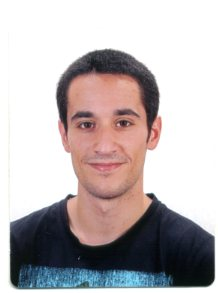
\includegraphics[width=0.6\columnwidth]{fede_fototessera.jpg}\\[\baselineskip] % Your photo
\small % Smaller font size
Federico Massa \\ % Your name
\url{fedemassa91@gmail.com}  \\
%\url{gmail.com} \\ % Your email address
%\url{www.johnsmith.com} \\ % Your URL
(+39) 347-7034248 \\ % Your phone number
\Sep % Some whitespace
\textbf{Address} \\
Via G. B. Pellizzi, 6 \\ % Address 1
56127 Pisa (PI) \\ % Address 2
Italy \\ % Address 3
\vfill % Whitespace under this block to push it up under the photo
\end{flushright}
}

%----------------------------------------------------------------------------------------

\begin{document}

\userinformation % Print your information in the left column

\framebreak % End of the first column

%----------------------------------------------------------------------------------------
%	HEADING
%----------------------------------------------------------------------------------------

\cvheading{Federico Massa} % Large heading - your name

\cvsubheading{Fisico} % Subheading - your occupation/specialization

%----------------------------------------------------------------------------------------
%	ABOUT ME
%----------------------------------------------------------------------------------------

%----------------------------------------------------------------------------------------
%	EDUCATION
%----------------------------------------------------------------------------------------

\CVSection{Istruzione}

%------------------------------------------------

\CVItem{2013 - 2016, Universit\`a di Pisa}{Laurea Magistrale in Fisica (curriculum Interazioni Fondamentali)\\ - 110/110 e lode.\\
- Titolo della tesi: ``Tracking performances of the ATLAS detector for the HL-LHC and impact on 
the H $\rightarrow 4\mu$ channel''.}

%------------------------------------------------


\CVItem{2010 - 2013, Universit\`a degli Studi di Cagliari}{Laurea Triennale in Fisica - 110/110 e lode.\\
- Titolo della tesi: ``Impact of physics beyond the Standard Model on the diffusion of neutrinos on polarized electrons''.}

%------------------------------------------------

\CVItem{2005 - 2010, Liceo Scientifico Pitagora - Selargius (CA)}{Diploma di Maturit\`a Scientifica - 100/100 e lode.}

\CVSection{Esperienze}

\CVItem{1 Novembre 2016 - 30 Gennaio 2017: Pisa}{Contratto di collaborazione occasionale con il Centro Ricerche E. Piaggio (Università di Pisa)}

\CVItem{5 - 10 Giugno 2016: Alghero}{Partecipazione al workshop \textit{XIII Seminar on Nuclear, Subnuclear and Applied Physics}}

\CVItem{20 Luglio - 1 Agosto 2014: Göttingen}{Partecipazione alla \textit{HASCO Summer School on Hadron Colliders}}
%\Sep % Extra whitespace after the end of a major section

%----------------------------------------------------------------------------------------
%	EXPERIENCE
%----------------------------------------------------------------------------------------

%\CVSection{Experience}

%------------------------------------------------

%------------------------------------------------

%------------------------------------------------

\Sep % Extra whitespace after the end of a major section

%----------------------------------------------------------------------------------------
%	COMMUNICATION SKILLS
%----------------------------------------------------------------------------------------
\CVSection{Competenze linguistiche}
\begin{table}[h!]
\centering
\resizebox{.71\textwidth}{!}{\tabulinesep=1.2mm{\begin{tabu}{| l | c | c | c | c | c |}
\cline{2-6}
\multicolumn{1}{c}{ } & \multicolumn{2}{|c|}{\textbf{Comprensione}} & \multicolumn{2}{c|}{\textbf{Orale}} & \textbf{Produzione scritta} \\ \cline{2-6}
\multicolumn{1}{c}{ } & \multicolumn{1}{|c|}{Ascolto} & Lettura & Interazione & Produzione \\ \hline
Inglese & C1 & C1 & C1 & C1 & C1 \\ \hline
Spagnolo & B2 & B2 & B2 & B2 & B2 \\ \hline
\end{tabu}}}
\end{table}

\Sep 

\CVSection{Abilità di comunicazione}

%------------------------------------------------

\CVItem{2015-2016, Presentazioni}{Durante il periodo di tesi della Laurea Magistrale, ho presentato il mio lavoro in numerose occasioni a diversi gruppi di ricerca dell'esperimento ATLAS:
 \begin{itemize}
 \item ATLAS Pisa;
 \item ITk Simulation \& Performance;
 \item Upgrade Tracking;
 \item Physics Upgrade;
 \item ITk Layout Taskforce.
 \end{itemize}
 }

%------------------------------------------------
\Sep
Ho una forte propensione ed un'esperienza pluriennale nell'assistenza allo studio della
Fisica e della Matematica a studenti dalla scuola media fino alla Laurea Triennale. \\

%------------------------------------------------

%\Sep % Extra whitespace after the end of a major section

%----------------------------------------------------------------------------------------
%	SKILLS
%----------------------------------------------------------------------------------------

\clearpage
\userinformation
\framebreak

\CVSection{Abilità specifiche}
\begin{itemize}
\item Modellizzazione e simulazione di sistemi robotici distribuiti e cooperanti;
\item Tecniche di coordinamento di veicoli;
\item Analisi matematica;
\item Meccanica classica e quantistica;
\item Elettromagnetismo;
\item Analisi statistica dei dati;
\item Tecniche sperimentali;
\item Fondamenti di elettronica digitale e analogica;
\item Simulazioni Monte Carlo;
\item Image processing e Computer Vision.
\end{itemize}

\Sep 

\CVSection{Abilità informatiche}

%------------------------------------------------

\CVItem{Programmazione}
{\begin{tabular}{p{0.2\textwidth} p{0.2\textwidth} p{0.2\textwidth}}
\bluebullet C++ &  \bluebullet Java & \bluebullet Shell Unix\\
\bluebullet Python &  \bluebullet Mathematica & \bluebullet MATLAB\\
\bluebullet Fortran 90 & \bluebullet Visual Basic & \bluebullet C\\
\bluebullet LaTeX
\end{tabular}}

%------------------------------------------------

\CVItem{Sistemi operativi}
{\begin{tabular}{p{0.2\textwidth} p{0.2\textwidth} p{0.2\textwidth}}
 \bluebullet Windows &  \bluebullet Unix/Linux & \bluebullet Android\\
\end{tabular}}

%-----------------------------------------------

\CVItem{Software utilizzati}
{\begin{tabular}{p{0.2\textwidth} p{0.2\textwidth} p{0.2\textwidth}}
 \bluebullet ROOT framework & \bluebullet Geant4 framework & \bluebullet Gnuplot \\
 \bluebullet Android Studio & \bluebullet Qt Creator & \bluebullet Eclipse \\
 \bluebullet Matlab e SimuLink & \bluebullet Texmaker (editor) & \bluebullet Mathematica
\end{tabular}}

Tra i vari linguaggi, ho una lunga esperienza di programmazione in C++ e Java.

%------------------------------------------------

\Sep % Extra whitespace after the end of a major section

%----------------------------------------------------------------------------------------
%	NEW PAGE DELIMITER
%	Place this block wherever you would like the content of your CV to go onto the next page
%----------------------------------------------------------------------------------------

%----------------------------------------------------------------------------------------
%	AWARDS
%----------------------------------------------------------------------------------------

%\CVSection{Awards}

%------------------------------------------------

%\CVItem{2010, \textit{Postgraduate Scholarship}, Cornell University}{Awarded to the top student in their final year of a Bachelors degree.}

%------------------------------------------------

%\Sep % Extra whitespace after the end of a major section

%----------------------------------------------------------------------------------------
%	INTERESTS
%----------------------------------------------------------------------------------------

\CVSection{Interessi}

%------------------------------------------------

\CVItem{Professionali}{Sviluppo Software e di App, Intelligenza Artificiale, 
Automazione, Simulazione di sistemi fisici e multi-agente.}

%------------------------------------------------

\CVItem{Personali}{Programmazione Arduino, Sviluppo di App per Android, Musica, piano jazz, batteria,  
mountain-bike, video-games.}

%------------------------------------------------

\Sep % Extra whitespace after the end of a major section

%----------------------------------------------------------------------------------------
\CVSection{Allegati}

\textit{Certificato di Laurea Triennale con esami}\\
\textit{Certificato di Laurea Magistrale con esami}\\
\textit{Certificato di lingua inglese}\\
\textit{Certificato di lingua spagnola}\\
\textit{Certificato di superamento del test finale al workshop ad Alghero}\\

\bigskip
\textit{Autorizzo il trattamento dei miei dati personali, ai sensi del D.lgs. 196 del 30 giugno 2003.}\\

\end{document}
